\documentclass{article}

\usepackage{fancyhdr}
\usepackage{extramarks}
\usepackage{amsmath}
\usepackage{amsthm}
\usepackage{amsfonts}
\usepackage{tikz}
\usepackage[plain]{algorithm}
\usepackage{algpseudocode}
\usepackage[utf8]{inputenc}
\usepackage[T1]{fontenc}
\usepackage{natbib}

\usetikzlibrary{automata,positioning}

%
% Basic Document Settings
%

\topmargin=-0.45in
\evensidemargin=0in
\oddsidemargin=0in
\textwidth=6.5in
\textheight=9.0in
\headsep=0.25in

\linespread{1.1}

\pagestyle{fancy}
%\lhead{\hmwkAuthorName}
%\chead{\hmwkClass\ (\hmwkClassInstructor\ \hmwkClassTime): \hmwkTitle}
\lhead{\hmwkClass: \hmwkTitle}
\rhead{\hmwkAuthorName}
\lfoot{\lastxmark}
\cfoot{\thepage}

\renewcommand\headrulewidth{0.4pt}
\renewcommand\footrulewidth{0.4pt}

\setlength\parindent{0pt}
\setlength{\parskip}{1em}

%
% Create Problem Sections
%

\newcommand{\enterProblemHeader}[1]{
    \nobreak\extramarks{}{Problem \arabic{#1} continued on next page\ldots}\nobreak{}
    \nobreak\extramarks{Problem \arabic{#1} (continued)}{Problem \arabic{#1} continued on next page\ldots}\nobreak{}
}

\newcommand{\exitProblemHeader}[1]{
    \nobreak\extramarks{Problem \arabic{#1} (continued)}{Problem \arabic{#1} continued on next page\ldots}\nobreak{}
    \stepcounter{#1}
    \nobreak\extramarks{Problem \arabic{#1}}{}\nobreak{}
}

\setcounter{secnumdepth}{0}
\newcounter{partCounter}
\newcounter{homeworkProblemCounter}
\setcounter{homeworkProblemCounter}{1}
%\nobreak\extramarks{Problem \arabic{homeworkProblemCounter}}{}\nobreak{}

%
% Homework Problem Environment
%
% This environment takes an optional argument. When given, it will adjust the
% problem counter. This is useful for when the problems given for your
% assignment aren't sequential. See the last 3 problems of this template for an
% example.
%
\newenvironment{homeworkProblem}[1][-1]{
    \ifnum#1>0
        \setcounter{homeworkProblemCounter}{#1}
    \fi
    \section{Problem \arabic{homeworkProblemCounter}}
    \setcounter{partCounter}{1}
    \enterProblemHeader{homeworkProblemCounter}
}{
    \exitProblemHeader{homeworkProblemCounter}
}

%
% Homework Details
%   - Title
%   - Due date
%   - Class
%   - Section/Time
%   - Instructor
%   - Author
%

\newcommand{\hmwkTitle}{Rapport intermédiaire}
\newcommand{\hmwkDueDate}{26 mars, 2017}
\newcommand{\hmwkClass}{MTH8408}
\newcommand{\hmwkClassTime}{}
\newcommand{\hmwkClassInstructor}{Professeur Dominique Orban}
\newcommand{\hmwkAuthorName}{André Phu-Van Nguyen, 1525972}
\renewcommand{\refname}{Références}

%
% Title Page
%

\title{
    \vspace{2in}
    \textmd{\textbf{\hmwkClass:\ \hmwkTitle}}\\
    \normalsize\vspace{0.1in}\small{Remis\ pour\ le\ \hmwkDueDate\ }\\
    \vspace{0.1in}\large{\textit{\hmwkClassInstructor\ \hmwkClassTime}}
    \vspace{3in}
}

\author{\textbf{\hmwkAuthorName}}
\date{}

\renewcommand{\part}[1]{\textbf{\large Part \Alph{partCounter}}\stepcounter{partCounter}\\}

%
% Various Helper Commands
%

% Useful for algorithms
\newcommand{\alg}[1]{\textsc{\bfseries \footnotesize #1}}

% For derivatives
\newcommand{\deriv}[1]{\frac{\mathrm{d}}{\mathrm{d}x} (#1)}

% For partial derivatives
\newcommand{\pderiv}[2]{\frac{\partial}{\partial #1} (#2)}

% Integral dx
\newcommand{\dx}{\mathrm{d}x}

% Alias for the Solution section header
\newcommand{\solution}{\textbf{\large Solution}}
\newcommand{\norm}[1]{\left\lVert#1\right\rVert}

% Probability commands: Expectation, Variance, Covariance, Bias
\newcommand{\E}{\mathrm{E}}
\newcommand{\Var}{\mathrm{Var}}
\newcommand{\Cov}{\mathrm{Cov}}
\newcommand{\Bias}{\mathrm{Bias}}

\begin{document}

\maketitle

\pagebreak

\section{Rappel de la problématique}

Ce projet consiste en l'étude et l'implémentation de l'article \textit{Minimum Snap Trajectory Generation and Control for Quadrotors} par Daniel Mellinger et Vijay Kumar \cite{Mellinger2011} qui propose un contrôleur et un générateur de trajectoires pour un véhicule aérien multirotor. Plus précisément, nous faisont une implémentation seulement de la partie génération de trajectoire par une méthode d'optimisation numérique.

Lors du suivi d'une trajectoire, une solution triviale est souvent utilisée qui consiste en l'interpolation en ligne droite entre chaque point de cheminement ou \textit{waypoint} (Mellinger utilise plutôt l'apellation \textit{keyframe}). Ceci est inneficace car la courbure infinie à chaque waypoint oblige le quadricoptère à s'arrêter avant de passer au prochain waypoint. Mellinger propose donc de modéliser une trajectoire optimale par un polynôme défini par parties entièrement lisse à travers les différents waypoints tout en satisfaisant des contraintes sur les vitesses et accélérations possibles du véhicule. Ce problème est résolu en le reécrivant en problème d'optimisation quadratique.

Tout dabord Mellinger démontre que la dynamique d'un quadricoptère a la propriété dêtre différentiellement plat. C'est-à-dire que les états et les entrées peuvent être exprimées par les sorties du système et leurs dérivées. Nous avons donc le vecteur de sorties plates
$$\sigma = [x, y, z, \psi]^T$$
où $r = [x, y, z]^T$ est la position du centre de masse dans le système de coordonnées du monde et $\psi$ l'angle de lacet. Rappelons nous que dans un repère main droite centré sur un corps rigide, l'axe $x$ pointe vers l'avant, $y$ vers la gauche et $z$ vers le haut. Les angles de rotation autour de ces axes sont le roulis (\textit{roll}), tangage (\textit{pitch}) et lacet (\textit{yaw}) respectivement. À fin de garder le projet simple, nous ne considérons pas les angles de roulis et de tangage dans le problème mais nous savons qu'il est possible de le faire pour exécuter des manoeuvres accrobatiques tel que voler à travers une fenêtre inclinée.

\begin{figure}[h]
	\centering
	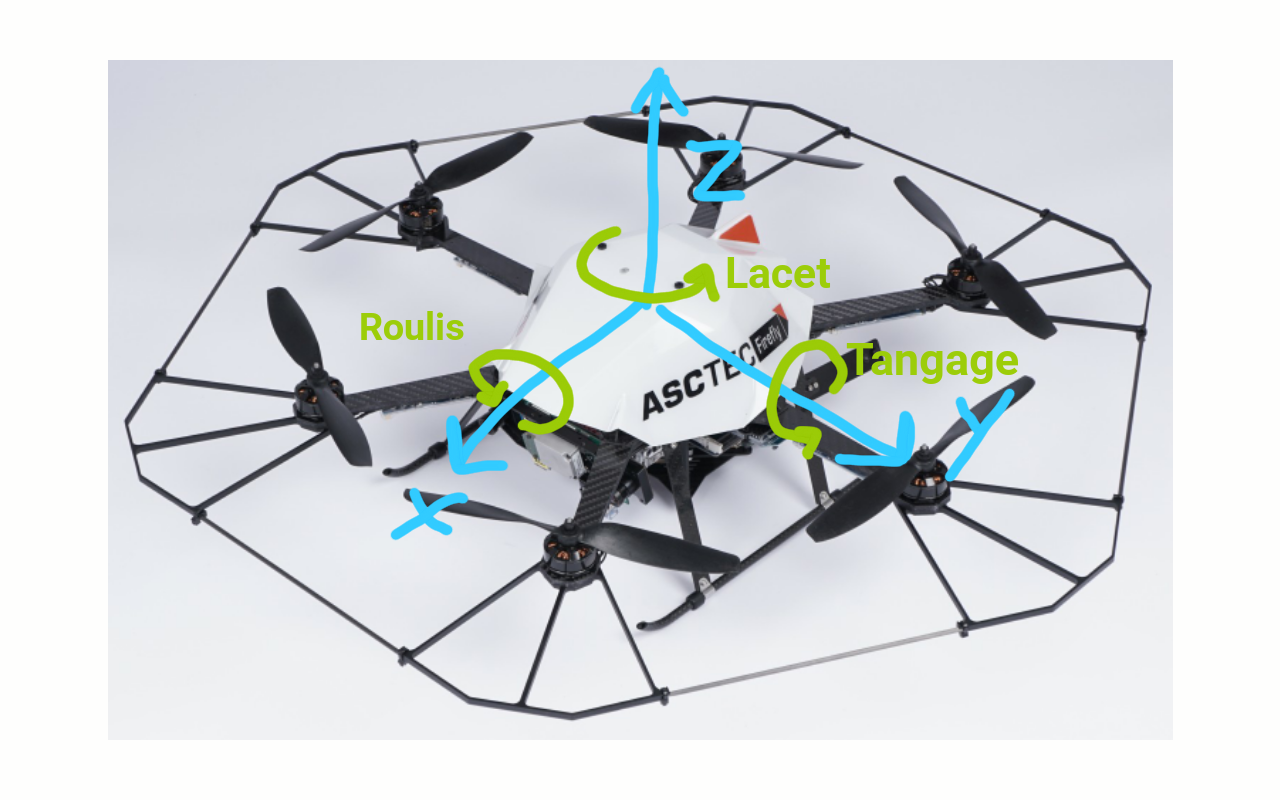
\includegraphics[width=0.5\textwidth]{fig/firefly.png}
	\caption{Systèmes de coordonnées d'un hexacoptère. L'angle de lacet est la rotation du véhicule autour de son axe Z, c'est-à-dire quand le véhicule tourne sur lui même.}
\end{figure}

Une trajectoire est définie comme était une courbe lisse dans l'espace des sorties plates:
$$ \sigma(t) : [t_0, t_m] \rightarrow \mathbb{R}^3 \times SO(2)$$
où $t_0$ et $t_m$ sont les temps de début et de fin de la trajectoire, $m$ correspond au nombre d'intervales de temps entre chaque waypoint et $SO(2)$ est le groupe spécial orthogonal. En pratique, une trajectoire est plutôt décrite par un polynôme défini par parties:
\begin{align}\label{eq:polynomial}
\sigma_T(t) =
\left\{
	\begin{array}{ll}
		\sum_{i=0}^n \sigma_{Ti1} t^i  & t_0 \leq t < t_1 \\
		\sum_{i=0}^n \sigma_{Ti2} t^i  & t_1 \leq t < t_2 \\
		... \\
		\sum_{i=0}^n \sigma_{Tim} t^i  & t_{m-1} \leq t < t_m \\
	\end{array}
\right.
\end{align}
où $n$ est l'ordre du polynôme et $m$ est encore le nombre d'intervales de temps.

Étant donné que l'on veut optimiser la dérivée d'ordre $k_r = 4$ (le \textit{snap}) de la position au carré et la dérivée d'ordre $k_\psi = 2$ (accélération angulaire) de langle de lacet $\psi$ au carré, nous avons le problème d'optimisation:
\begin{align}\label{eq:opt}
\text{min} \int_{t_0}^{t_m} \mu_r \norm{\frac{d^4 \boldsymbol{r}_T}{dt^4}}^2 + \mu_\psi {\ddot{\psi}_T}^2 dt
\end{align}\begin{align*}
	\begin{array}{lll}
%		\text{sous contraintes} & \sigma_T(t_i) = \sigma_i & i = 0, \ldots, m\\
		\text{sous contraintes} & \boldsymbol{r}_T(t_i) = \boldsymbol{r}_i & i = 0, \ldots, m\\
		& \psi_T(ti)=\psi_i & i = 0, \ldots, m\\
		& \frac{d^p x_T}{dt^p}|_{t=t_j} = 0\ \text{ou libre,} & j = 0, m; p = 1, 2, 3, 4\\
		& \frac{d^p y_T}{dt^p}|_{t=t_j} = 0\ \text{ou libre,} & j = 0, m; p = 1, 2, 3, 4\\
		& \frac{d^p z_T}{dt^p}|_{t=t_j} = 0\ \text{ou libre,} & j = 0, m; p = 1, 2, 3, 4\\
		& \frac{d^p \psi_T}{dt^p}|_{t=t_j} = 0\ \text{ou libre,} & j = 0, m; p = 1, 2\\
	\end{array}
\end{align*}

où $\boldsymbol{r}_T = [x_T, y_T, z_T]^T$ et $r_i = [x_i, y_i, z_i]$.

\section{Changements à la problématique}

Puisque les implémentations initiales ne fonctionnaient pas (la trajectoire semblait diverger et ne respectait pas les contraintes imposées) nous avons fait quelques changements à la problématique pour simplifier les choses pour au moins obtenir une solution fonctionnelle avant de l'améliorer. Tout d'abord nous avons retiré l'angle de lacet du problème. Ensuite nous avons remarqué que Mellinger indique dans son article que les états sont découplées dans leurs fonction de coût et leurs contraintes alors en pratique nous pouvons séparer le problème en plusieurs sous problèmes d'optimisation. Au final la génération de trajectoire se fait donc par l'optimisation de trois problèmes quadratiques pour les dimensions $x$, $y$ et $z$. Par exemple pour la trajectoire en $x$ nous avons

\begin{align}\label{eq:opt_x}
\text{min} \int_{t_0}^{t_m} \mu_r \norm{\frac{d^4 \boldsymbol{x}_T}{dt^4}}^2 dt
\end{align}\begin{align*}
	\begin{array}{lll}
%		\text{sous contraintes} & \sigma_T(t_i) = \sigma_i & i = 0, \ldots, m\\
		\text{sous contraintes} & \boldsymbol{x}_T(t_i) = \boldsymbol{x}_i & i = 0, \ldots, m\\
		& \frac{d^p x_T}{dt^p}|_{t=t_j} = 0\ \text{ou libre,} & j = 0, m; p = 1, 2, 3, 4
	\end{array}
\end{align*}

où $\boldsymbol{x}_T$ est le vecteur contenant les coefficients du polynôme représentant la trajectoire dans la dimension $x$.

\section{Structure du problème d'optimisation}

Puisque l'article de Mellinger comporte très peu de détails et ne discute de la manière de poser le problème que vaguement, nous avons été obligé de faire le développement des équations à la main et au final nous avons aussi été obligé de consulter d'autres articles (Bry et Richter) citant celui de Mellinger pour mieux comprendre comment faire. Le dévelppement mathématique suivant est donc un mélange de notre propre travail et de ce qui est écrit dans \cite{Richter2016, bry2012control}.

Considérons le problème en une dimension $p$, où $p = x$, $y$ ou $z$. Nous pouvons reformuler le problème en tant que problème d'optimisation quadratique en réécrivant les coefficients des polynômes en un vecteur $c$ de dimension $4m \times 1$, où $m$ est le nombre de waypoints en excluant les conditions initiales. Nous obtenons la forme standard:
\begin{align}\label{eq:opt_quad}
\text{min}\ \ \ c^THc+f^Tc
\end{align}\begin{align*}
	\begin{array}{ll}
	\text{s. c.} & Ac = b
	\end{array}
\end{align*}

Avant de construire la matrice $H$ nous devons développer les équations des polynômes représentant un segment de trajectoire i.e. la trajectoire entre deux waypoints. En réglant l'ordre du polynôme à $n = 6$ nous avons pour un axe de déplacement $p$ en 3D où $p = x$, $y$ ou $z$:
\begin{align*}
\boldsymbol{p} &= c_6 t^6 + c_5 t^5 + c_4 t^4 + c_3 t^3 + c_2 t^2+ c_1 t + c_0\\
\frac{d \boldsymbol{p}}{dt} &= 6 c_6 t^5 + 5 c_5 t^4 + 4 c_4 t^3 + 3 c_3 t^2 + 2c_2 t + c_1 + 0\\
\frac{d^2 \boldsymbol{p}}{dt^2} &=
	(6\cdot 5) c_6 t^4 + (5 \cdot 4) c_5 t^3 + (4 \cdot 3) c_4 t^2 + (3 \cdot 2) c_3 t + 2c_2 + 0 + 0\\
\frac{d^3 \boldsymbol{p}}{dt^3} &=
	(6\cdot 5\cdot 4) c_6 t^3 + (5 \cdot 4\cdot 3) c_5 t^2 + (4 \cdot 3\cdot 2 ) c_4 t + (3 \cdot 2) c_3 + 0 + 0 + 0\\
\frac{d^4 \boldsymbol{p}}{dt^4} &=
	(6\cdot 5\cdot 4\cdot 3) c_6 t^2 + (5 \cdot 4\cdot 3\cdot 2) c_5 t + (4 \cdot 3\cdot 2 ) c_4 + 0 + 0 + 0 + 0\\
\end{align*}
Prendre la norme euclidienne au carré de la position est équivalent à prendre le carré de chaque polynôme. Donc pour un polynôme $p$ représentant un axe $x$, $y$ ou $z$ nous avons:
\begin{align}\label{eq:polynome_derive}
\norm{\frac{d^4 \boldsymbol{p}}{dt^4}}^2 &=
	\bigg((6\cdot 5\cdot 4\cdot 3) c_6 t^2 + (5 \cdot 4\cdot 3\cdot 2) c_5 t + (4 \cdot 3\cdot 2 ) c_4 \bigg)^2 \\
	&=	(6\cdot 5\cdot 4\cdot 3)^2 c_6^2 t^4 + (6\cdot 5\cdot 4\cdot 3)(5 \cdot 4\cdot 3\cdot 2) c_6 c_5 t^3 + (6 \cdot 5 \cdot 4\cdot 3)(4\cdot 3\cdot 2)c_6 c_4 t^2 \nonumber\\
	&	+ (5 \cdot 4\cdot 3\cdot 2)^2 c_5^2 t^2 + (6\cdot 5\cdot 4\cdot 3)(5 \cdot 4\cdot 3\cdot 2) c_6 c_5 t^3 + (5 \cdot 4\cdot 3\cdot 2)(4\cdot 3\cdot 2)c_5 c_4 t \nonumber\\
	&	+ (4\cdot 3\cdot 2)^2 c_4^2 + (6 \cdot 5 \cdot 4\cdot 3)(4\cdot 3\cdot 2)c_6 c_4 t^2 + (5 \cdot 4\cdot 3\cdot 2)(4\cdot 3\cdot 2)c_5 c_4 t \nonumber\\
	& = (6\cdot 5\cdot 4\cdot 3)^2 c_6^2 t^4 + 2(6\cdot 5\cdot 4\cdot 3)(5 \cdot 4\cdot 3\cdot 2) c_6 c_5 t^3 + 2(6 \cdot 5 \cdot 4\cdot 3)(4\cdot 3\cdot 2)c_6 c_4 t^2 \nonumber\\
	&	+ (5 \cdot 4\cdot 3\cdot 2)^2 c_5^2 t^2 + 2 (5 \cdot 4\cdot 3\cdot 2)(4\cdot 3\cdot 2)c_5 c_4 t \nonumber\\
	&	+ (4\cdot 3\cdot 2)^2 c_4^2 \nonumber
\end{align}

Ensuite, pour un waypoint $j$ nous avons le temps de départ $t_j$ et le temps d'arrivée au prochain waypoint $t_{j+1}$, nous pouvons écrire le résultat de l'intégrale:
\begin{align}\label{eq:polynome_integre}
\int_{t_j}^{t_{j+1}} \norm{\frac{d^4 \boldsymbol{p}}{dt^4}}^2 dt
	& = \int_{t_j}^{t_{j+1}} (6\cdot 5\cdot 4\cdot 3)^2 c_6^2 t^4 + 2(6\cdot 5\cdot 4\cdot 3)(5 \cdot 4\cdot 3\cdot 2) c_6 c_5 t^3 \\
	&	+ 2(6 \cdot 5 \cdot 4\cdot 3)(4\cdot 3\cdot 2)c_6 c_4 t^2 + (5 \cdot 4\cdot 3\cdot 2)^2 c_5^2 t^2 + 2(5 \cdot 4\cdot 3\cdot 2)(4\cdot 3\cdot 2)c_5 c_4 t \nonumber \\
	&	+ (4\cdot 3\cdot 2)^2 c_4^2 \ dt\nonumber \\
%	&= (6\cdot 5\cdot 4\cdot 3)^2 c_6^2 \frac{1}{4} t^3 \Big|_{t_j}^{t_{j+1}} + 2(6\cdot 5\cdot 4\cdot 3)(5 \cdot 4\cdot 3\cdot 2) c_6 c_5 \frac{1}{3} t^2\Big|_{t_j}^{t_{j+1}}\nonumber \\
%	&	+ 2(6\cdot 5\cdot 4\cdot 3)(4\cdot 3\cdot 2) c_6 c_4 \frac{1}{2} t\Big|_{t_j}^{t_{j+1}}
%		+ (5 \cdot 4\cdot 3\cdot 2)^2 c_5^2 \frac{1}{2} t\Big|_{t_j}^{t_{j+1}} \nonumber \\
	&=	360^2 c_6^2 \frac{1}{5} t^5 \Big|_{t_j}^{t_{j+1}}
		+ 2 \cdot 360 \cdot 120 c_6 c_5 \frac{1}{4} t^4\Big|_{t_j}^{t_{j+1}}
		+ 2 \cdot 360 \cdot 24 c_6 c_4 \frac{1}{3} t^3\Big|_{t_j}^{t_{j+1}} \nonumber \\
	&	+ 120^2 c_5^2 \frac{1}{3} t^3\Big|_{t_j}^{t_{j+1}} + 2 \cdot 120 \cdot 24 c_5 c_4 \frac{1}{2}t^2 \Big|_{t_j}{t_{j+1}} \nonumber \\
	&	+ 24^2 c_4^2 t\Big|_{t_j}^{t_{j+1}} \nonumber
\end{align}


Avec le résultat en (\ref{eq:polynome_integre}) on peut maintenant poser une partie de la matrice $H$ de (\ref{eq:opt_quad}).

Tel qu'indiqué précédemment, le vecteur $c$ contient tous les coefficients de tous les polynômes de chaque segment de la trajectoire et de chaque degré de liberté. La partie de $c$ correspondant à un axe $p$ est donc $[c_6,\ c_5,\ c_4,\ c_3,\ c_2,\ c_1,\ c_0]^T$. Par conséquent, nous pouvons déduire la matrice $H_{pj}$ correspondante pour un waypoint $j$
\begin{align}\label{eq:hessienne_p}
H_{pj} =
\begin{bmatrix}
    360^2 \frac{1}{5} t^5 \Big|_{t_j}^{t_{j+1}}
    		& 2 \cdot 360 \cdot 120 \frac{1}{4} t^4\Big|_{t_j}^{t_{j+1}}
    		& 2 \cdot 360 \cdot 24 \frac{1}{3} t^3\Big|_{t_j}^{t_{j+1}}
    		& 0
    		& 0
    		& 0
	    	& 0 \\
    2 \cdot 360 \cdot 120 \frac{1}{4} t^4\Big|_{t_j}^{t_{j+1}}
    		& 120^2 \frac{1}{3} t^3\Big|_{t_j}^{t_{j+1}}
    		& 2 \cdot 120 \cdot 24 \frac{1}{2}t^2 \Big|_{t_j}^{t_{j+1}} & 0 & 0 & 0 & 0\\
	2 \cdot 360 \cdot 24 \frac{1}{3} t^3\Big|_{t_j}^{t_{j+1}}
		& 2 \cdot 120 \cdot 24 \frac{1}{2}t^2 \Big|_{t_j}^{t_{j+1}}
		& 24^2 t\Big|_{t_j}^{t_{j+1}} & 0 & 0 & 0 & 0 \\
    0 & 0 & 0 & 0 & 0 & 0 & 0 \\
    0 & 0 & 0 & 0 & 0 & 0 & 0 \\
    0 & 0 & 0 & 0 & 0 & 0 & 0 \\
    0 & 0 & 0 & 0 & 0 & 0 & 0 \\
\end{bmatrix}
\end{align}

Bien que Mellinger ne le présente pas dans son article, Richter et Bry \cite{Richter2016, bry2012control} indiquent que ce processus peut être automatisé par la formule suivante:
\begin{align}
H_{pj} =\left\{
  \begin{array}{ll}
    2 \Big( \prod_{m = 0}^{r-1} (i-m)(l-m)\Big) \frac{\tau^{i+l-2r+1}}{i+l-2r+1}: & i \geq r \text{ ou } l \geq r \\
    0 : & \text{autrement}
  \end{array}
  \right.
\end{align}
où $i$ et $l$ sont les index de rangée et de colonne et $\tau$ est la durée du segment de trajectoire.

\subsection{Structure de la matrice H finale}

Une fois le développement précédent fait, nous pouvons concaténer en diagonale les matrices $H_{pj}$ pour chaque waypoint jusqu'à $j=m$, pour chaque waypoint jusqu'au dernier waypoint $j=m$ pour former $H$ de (\ref{eq:opt_quad}).

\begin{align}
H_x=
\begin{bmatrix}
	H_{x1} \\
	&	H_{x2} \\
	&	&		\ddots \\
	&	&		&		H_{xm}
\end{bmatrix}
\end{align}

De plus, par le développement précédent en (\ref{eq:polynome_integre}), nous pouvons voir que le terme linéaire $f^Tc$ de (\ref{eq:opt_quad}) est nul.

\subsection{Structure des matrices de contraintes A et b}

Dans ce problème nous utilisons les matrices de contraintes d'égalité de deux façons. Premièrement pour imposer la valeur d'une certaine dérivée à un certain moment et deuxièmement pour imposer la continuité entre deux segments de trajectoire.

Dans notre code, nous avons appelé ceci les contraintes de départ et d'arrivée et les contraintes de continuité. Encore une fois, nous suivons la formulation de Bry \cite{bry2012control}(car Mellinger donne peu de détails dans son article) où pour un segment de trajectoire allant du temps $0$ au temps $\tau$ nous pouvons contruire $A$ et $b$ de telle manière que
\begin{align}
A = \begin{bmatrix} A_0 \\ A_\tau \end{bmatrix},\ \ b = \begin{bmatrix} b_0 \\ b_\tau \end{bmatrix}
\end{align}
\begin{align}
A_{0_{rn}} = \left\{
  \begin{array}{ll}
    \prod_{m = 0}^{r-1} (r-m): & r = n \\
    0 : & \text{autrement}
  \end{array}
\right.
\end{align}
\begin{align}
b_{0_r} = P^{(r)}(0)
\end{align}
\begin{align}
A_{\tau_{rn}} = \left\{
  \begin{array}{ll}
    \big(\prod_{m = 0}^{r-1} (n-m) \Big) \tau^{n-r} : & n \geq r \\
    0 : & \text{autrement}
  \end{array}
\right.
\end{align}
\begin{align}
b_{\tau_r} = P^{(r)}(\tau)
\end{align}

Notons que $A_0$ et $A_\tau$ ont $r+1$ rangées (une par dérivée incluant la dérivée 0) et $n$ colonnes (une par coefficient du polynôme). La notation $P^{(r)}(0)$ indique le polynôme dérivé au degré $r$ et évalué au temps $0$. Si jamais la dérivée est sans contrainte, par exemple si nous ne boulons pas imposer la valeur de l'accélération à un certain waypoint, il suffit simplement d'ommettre la ligne correspondante de la matrice $A$.

En appliquant les équations précédentes, nous imposons à chaque waypoint une valeur fixe pour la position, la vitesse, le \textit{jerk} et le \textit{snap}. Tant à l'arrivée qu'au départ de celui ci. Par contre, si jamais l'utilisateur n'impose pas de contraintes sur ces dérivées, il faut tout de même ajouter des contraintes de continuité pour imposer que la valeur calculée (par le processus d'optimisation) pour cette dérivée soit continue au waypoint. Pour ce faire, il suffit de mettre égal les deux polynômes représentant les segments de part et d'autre d'un waypoint. Soit le polynôme dérivé $r$ fois allant au waypoint $j$, $P_{j}^{(r)}$ et le prochain polynôme partant du waypoint $j$, $P_{j+1}^{(r)}$ nous avons la contrainte

\begin{align*}
	P_{j}^{(r)} &= P_{j+1}^{(r)}\\
	-P_{j+1}^{(r)} + P_{j}^{(r)} &= 0
\end{align*}

Par inspection, nous pouvons recouvrir la forme de $A$ finale proposée par Bry \citep{bry2012control}. Prenons la notation $A_0^j$ la matrice de contraintes pour un début de trajectoire au waypoint $j$ et de même pour $A_\tau^j$ la matrice de contraintes pour une fin de trajectoire au waypoint $j$. Nous avons au final:
\begin{align}
A=  \begin{bmatrix}
		A_0^0	& 0	& 0 & 0 & \ldots & 0 & 0 \\
		-A_\tau^0 & A_0^1 & 0 & 0 & \ldots & 0 & 0 \\
		0 &  -A_\tau^1 & A_0^2 & 0 & \ldots & 0 & 0\\
		0 & 0 & -A_\tau^2 & A_0^3 & \ldots &0 &0 \\
		\ldots & \ldots & \ldots & \ldots & \ddots & \ldots & \ldots \\
		0& 0& 0& 0& 0& -A_\tau^{m-1} & A_0^m \\
				0& 0& 0& 0& 0& 0& A_\tau^m
	\end{bmatrix}
\end{align}
\begin{align}
b = \left\{
  \begin{array}{ll}
    \text{Valeur de la dérivée du polynôme $P$ imposée}: & \text{Si imposé} \\
    0 : & \text{autrement}
  \end{array}
\right.
\end{align}

\section{Structure du deuxième problème d'optimisation}

Mellinger montre que si jamais le temps d'arrivé à chaque segment n'importe pas, il est possible dans un deuxième temps de résoudre un deuxième problème d'optimisation à fin de trouver la meilleur répartition de temps possible entre chaque segment de la trajectoire.

Au lieu de considérer les temps d'arrivés $t_i$ à un waypoint $i$, nous pouvons plutôt considérer le temps de durée d'un segment de trajectoire $T_i = t_i - t_{i-1}$ et $T = [T_0, T_1, ..., T_i]$. Soit $f(T) = f_x(T) +  f_y(T) + f_z(T)$, la somme des valeurs de fonction de coût après la résolution du problème (\ref{eq:opt_x}) dans chaque dimension. Nous résolvons maintenant le problème
\begin{align}\label{eq:time_opt}
\text{min}\ \ \ f(T)
\end{align}\begin{align*}
\begin{array}{lll}
\text{s. c.} & \sum T_i = t_m & i = 1,\ldots,m\\
& T_i \geq 0 &  i = 1,\ldots,m\\
\end{array}
\end{align*}
où $T_i = t_i - t_{i-1}$ sont les temps alloués à chaque segment de la trajectoire. Il est relativement trivial de reécrire le problème sous la forme standard
\begin{align*}
\text{min}\ \ \ f(x)\\
\begin{array}{lll}
\text{s. c.} & Ax = b\\
& \text{lb} \leq x\\
\end{array}
\end{align*}
$A$ est de taille $1 \times m$ avec des $1$ partout $b = t_m$ le temps d'arrivé au dernier waypoint et lb$=0$. 

Par contre, ce qui est un peu moins trivial est la façon de fournir le gradient de $f(T)$ à la fonction d'optimisation. Mellinger le calcule numériquement par l'équation
\begin{align}
	\nabla_{g_i}f = \frac{f(T + hg_i) - f(T)}{h}
\end{align}
où h est une "petite" valeur et le vecteur colonne\footnote{Mellinger utilse en fait $\frac{-1}{m-2}$ car son $m$ inclut aussi les conditions initiales.} 
\begin{align}
g_i = \left\{
  \begin{array}{ll}
    1: & \text{à la position }i  \\
    \frac{-1}{m-1} : & \text{autrement}
  \end{array}
\right.
\end{align}
par exemple, dans le cas où $m=3$ nous aurions
\begin{align*}
	g_1 = \begin{bmatrix} 1\\ -\frac{1}{2} \\-\frac{1}{2} 	\end{bmatrix}\text{, }
	g_2 = \begin{bmatrix} -\frac{1}{2}\\ 1 \\-\frac{1}{2} 	\end{bmatrix}\text{ et }
	g_3 = \begin{bmatrix} -\frac{1}{2} \\-\frac{1}{2}\\ 1 	\end{bmatrix}
\end{align*}
et le gradient final serait
\begin{align*}
\nabla f = \begin{bmatrix}
	\nabla_{g_1}f\\
	\nabla_{g_2}f\\
	\nabla_{g_3}f\\
\end{bmatrix} = \begin{bmatrix}
	 \frac{f(T + hg_1) - f(T)}{h}\\
	 \frac{f(T + hg_2) - f(T)}{h}\\
	 \frac{f(T + hg_3) - f(T)}{h}\\
\end{bmatrix}
\end{align*}















\bibliographystyle{abbrv}
\bibliography{bibliography}

\end{document}
